\section{SP4RR - Serial Protocol for Rolling Road}
\label{sec:UART}
\fxnote{Missing introduction}
Each command is termintad by a newline character, and each value in a command is separated by a whitespace. \\

Overview of types:
\begin{table}[h!]
	\centering
	\label{Protocol:typeoverview}
	\begin{tabularx}{\linewidth}{p{1.5cm}Xp{3.5cm}}
		Type 	& Description 									& Example(s)    				\\\hline
		int  	& Signed integer that encoded in ASCII			& 0, 100 						\\
		string  & ASCII-encoded zero-terminated string 			& "RollingRoad"					\\ 
		float  	& Signed floating point number encoded in ASCII, where the decimals is seperated by ".". Int's is also a legal float      		& 100, 400.34 \\
	\end{tabularx}
	\caption{Overview for commands sent between PSoC og PC}
\end{table}

Overview of packets: \fxnote{Fix table}
\begin{table}[h!]
	\centering
	\label{Protocol:overviewRR}
	\begin{tabular}{l|llll}
		\# & Description 		& Command    		& Direction             & Example     		\\\hline
		0  & Handshake   		& RollingRoad 		& PC $\rightarrow$ PSoC & 0 RollingRoad 	\\
		1  & Type description 	& <int> <str> <str> & PSoC $\rightarrow$ PC & 1 0 Time Seconds 	\\
		2  & Stop        		&            		& PC $\rightarrow$ PSoC	& 2        			\\
		3  & Information 		& <double> ... <double>	& PSoC $\rightarrow$ PC & 3 2 3 	    	\\
		4  & Torque control 	& <double>    			& PC $\rightarrow$ PSoC & 4 0.5  				\\
		5  & PID control        & <double(P)> <double(I)> <double(D)> & PC $\leftrightarrow$ PSoC & 5 2.3 3.4 4.5 \\
		6  & Calibrate			&					& PC $\rightarrow$ PSoC & 6 \\ 
		7  & Reset distance meter & 				& PC $\rightarrow$ PSoC & 7 \\ 
		8  & Force control		& <double>    			& PC $\rightarrow$ PSoC & 8 12.5  				\\
	\end{tabular}
	\caption{Overview for commands sent between PSoC and PC}
\end{table}

\fxnote{Synes alle burde have eksempler - JH}

The table \ref{Protocol:overviewRR} will give an overview regarding the protocol that will be used between PC and PSoC. The chosen protocol will always start by sending an integer that corresponds with the given number from the above table.  The next thing that will be send is the column "Commando" that corresponds with the given number. The direction column shows the direction of the signals, where from and where to the signal will flow.

\subsection{Handshake}
The handshake command is used to establish that the connection between the PC and the embedded platform is correct. This is to ensure that it will not register an arbitrary unit and for that unit to send values to the PC.  

\textbf{Command layout:}

"0\textvisiblespace RollingRoad"

\subsection{Type description}
The type description command will give the PC 3 kinds of information. The first character in the transmitted message will be the command number, here 1. The first real information sent here\fxnote{Omformuler - JH}, relates to the information command. The integer here sent, will define the place of the information in the information packet that is sent. The next thing that will be sent is the tpye the PC can expect, fx. time, torque etc. The final thing that will be send is the unit for this particular information.

\textbf{Command layout:}

"1\textvisiblespace <Index>\textvisiblespace <Type-name>\textvisiblespace <Type-unit>"

\begin{table}[h!]
	\centering
	\label{Protocol:SP4RR_TypeDescVars}
	\begin{tabular}{llll}
		Value name 	& Type 		& Description 					& Contraints  					\\\hline
		Index  		& int   	& Index used when sending data 	& Equal or greather than zero	\\
		Type-Name  	& string 	& Name of index 				& No spaces						\\
		Type-Unit  	& string	& Unit of index					& No spaces 					\\
	\end{tabular}
	\caption{Overview of type description variables}
\end{table}

\subsection{Stop}
The stop command is used for stopping the data transmission. The stop command is called either by pressing a button on the GUI or closing the program on the PC.
When stop command is issued and data transmission is once again wanted, the protocol will start from the top, by sending the handshake command again. 

\textbf{Command layout:}

"2"

\subsection{Information}
The information command will be where all the information will be sent. Meaning that this command is going to be sent rapidly should be as short as possible. This is done by sending only the information needed, which is just the values of the information. To ensure that the PC and the PSoC communicates correctly here, the unit description command is used. \fxnote{Dem der læser dokumentationen kan vel næsten være ligeglade med hvorfor den er som den er, det skal bare vide hvordan de kan bruge den - JH}

\subsection{Torque control}
The torque control command  can change the input to the regulator. This is to change how much the generator is loaded and thereby how much the engine is strained. This parameter can be changed on the GUI. 

\subsection{PID control}
PID control is used to control the P, I and D parameters of the regulator. These parameters can then be adjusted during runtime. Furthermore the latest regulator parameters will be saved on an EEPROM on the PSoC, which will be send to the PC on startup. This is done to ensure the PC have updated numbers to start with.
          

In figure \ref{fig:SeqDiagram}, the flow of communication can be seen.
Starting with the handshake initiated by the PC, replying with unit descriptions for this transfer. When the connection is established after the handshake, the PSoC will send the information with a frequency of 10 Hz. On the GUI, the user can choose to regulate the torque, which then will be send and understood on the PSoC. Furthermore, the user have the ability to stop the data transfer, by pressing the stop button or by closing the program. When the command Stop is send, the PSoC will cease the data transfer.

\fxnote{Skal vidst opdateres med alle de nye commandoer}
\begin{figure}[h]
	\centering
	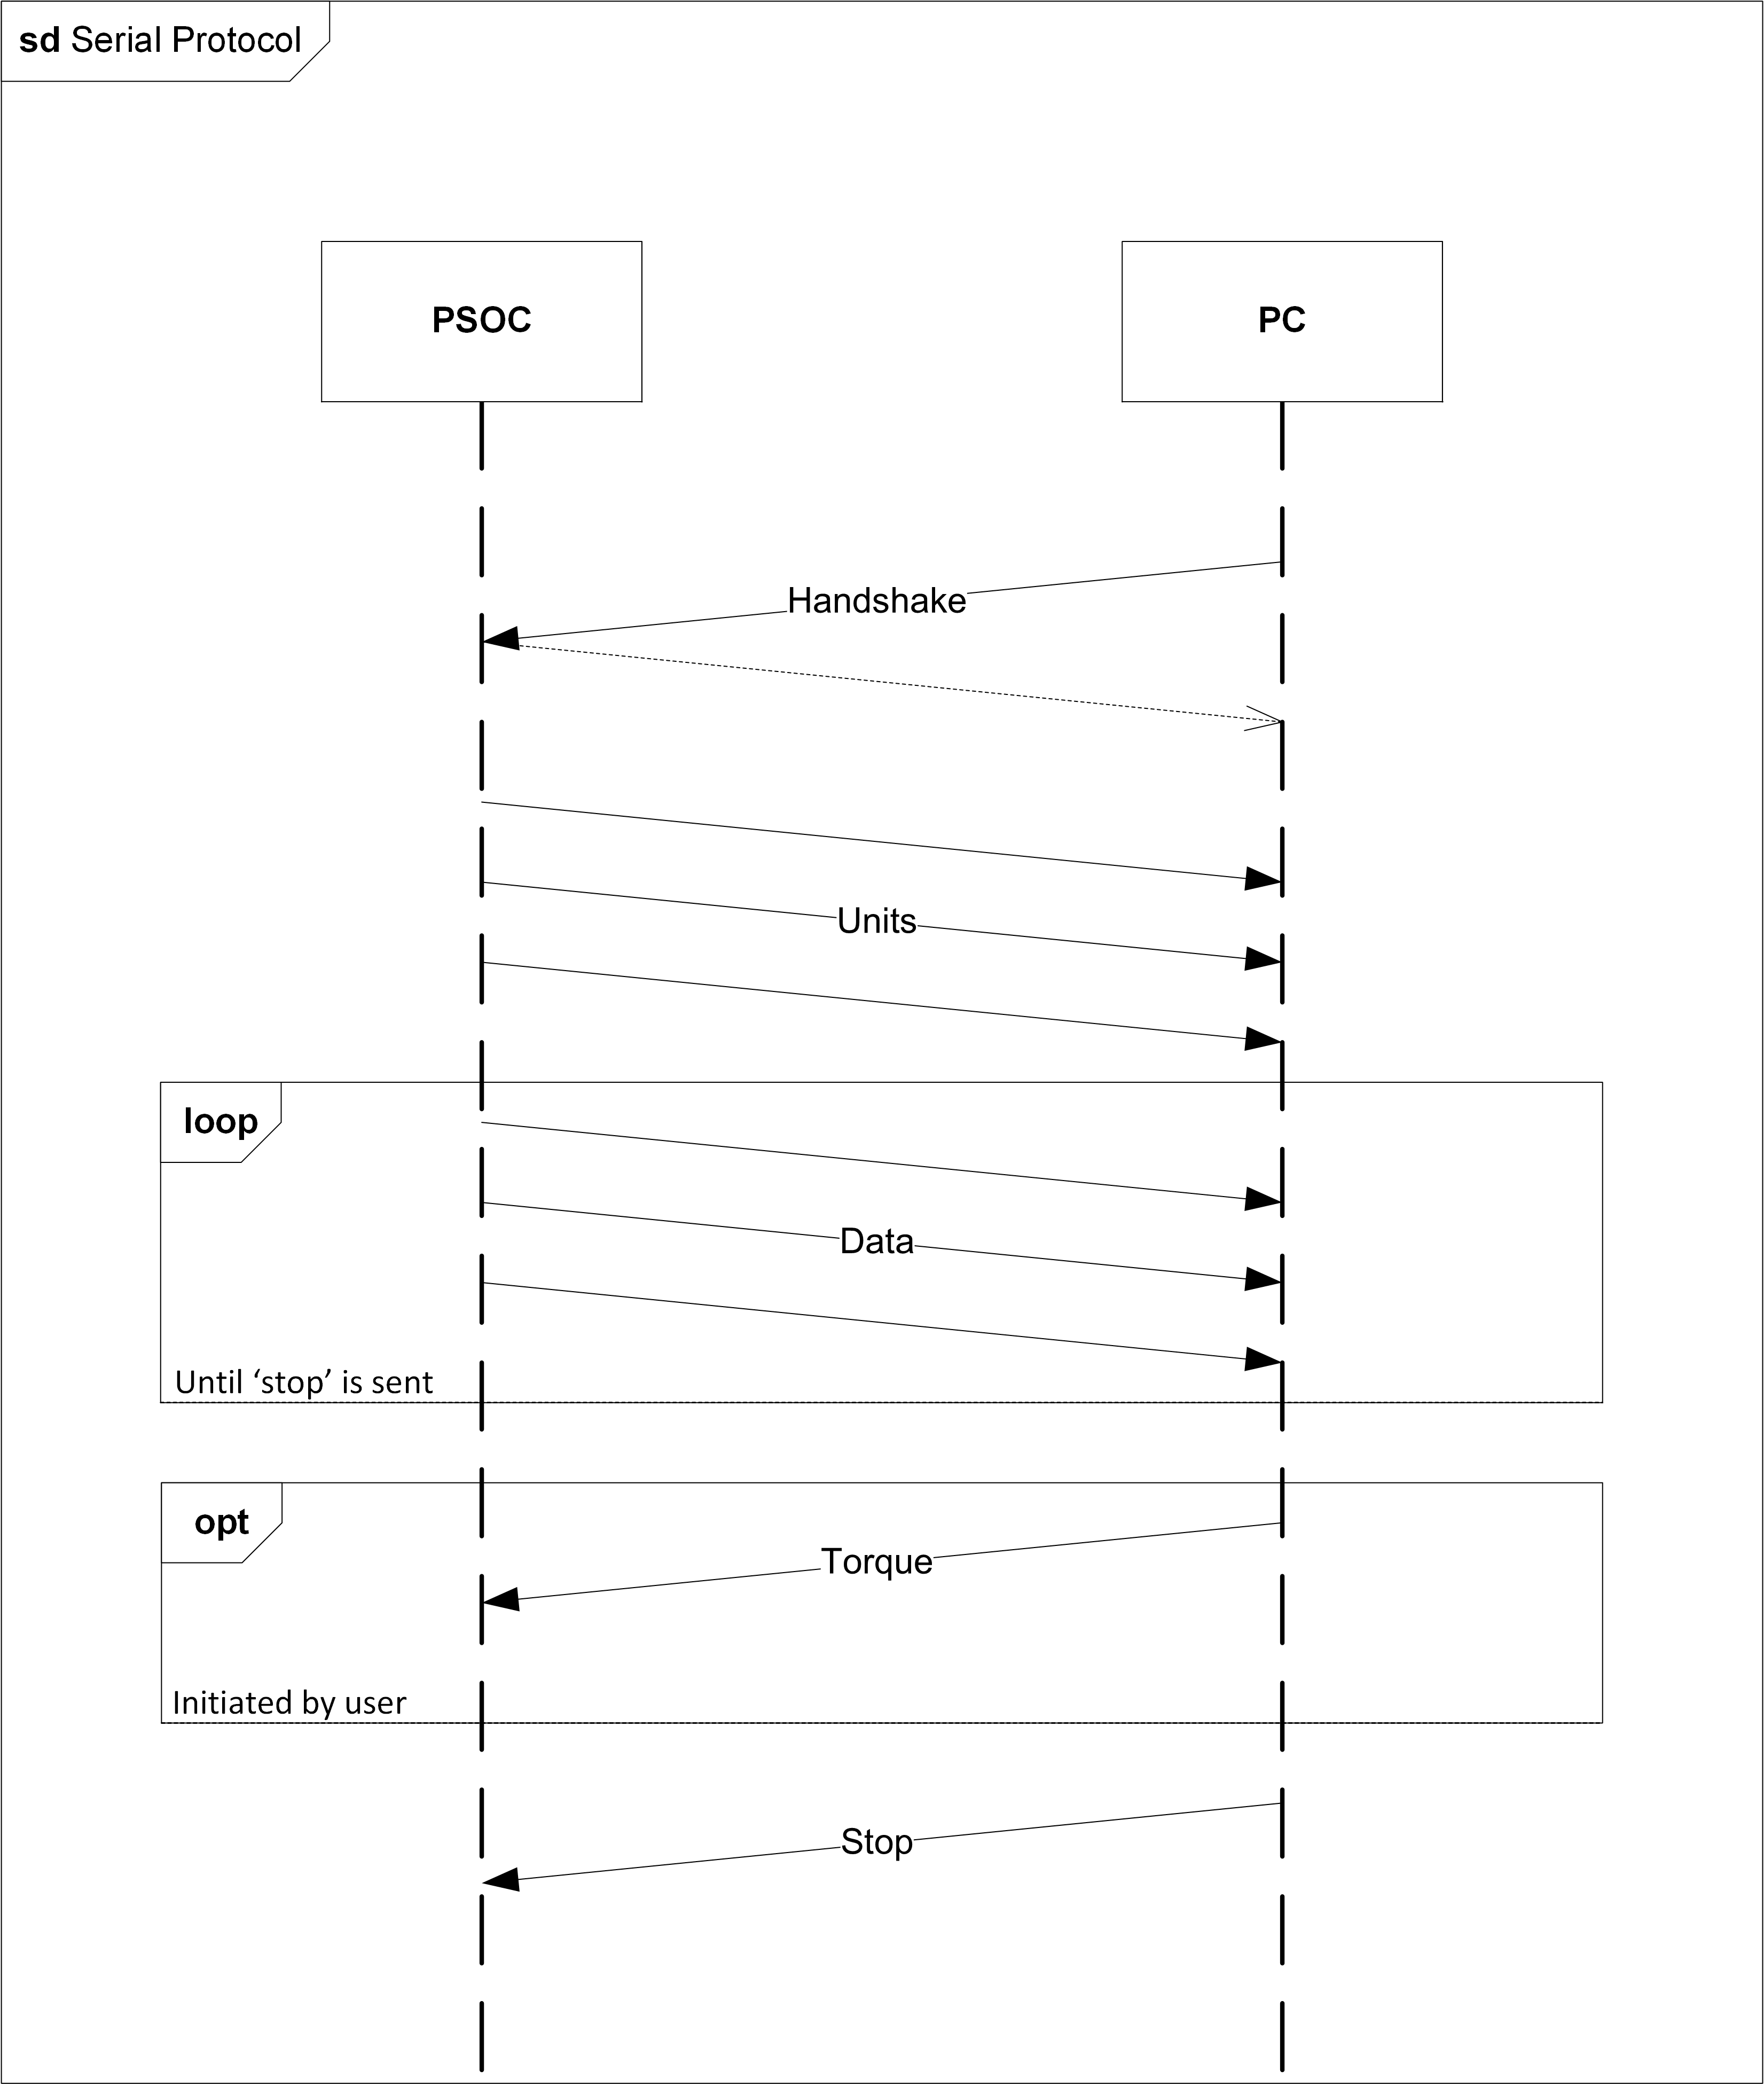
\includegraphics[width=1\linewidth]{Protocol/SD_Protocol}
	\caption{Sequence Diagram of the protocol}
	\label{fig:SeqDiagram}
\end{figure}

